\documentclass[11pt,letterpaper]{exam}
\usepackage[utf8]{inputenc}
\usepackage[spanish]{babel}
\usepackage{graphicx}
\usepackage{tabularx}
\usepackage[absolute]{textpos} % Para poner una imagen en posiciones arbitrarias
\usepackage{multirow}
\usepackage{float}
\usepackage{hyperref}
\usepackage[utf8x]{inputenc} 
\usepackage[normalem]{ulem}
\useunder{\uline}{\ul}{}
\usepackage[usenames]{color}
\title{Tarea 2 Métodos Computacionales\\\\ Departamento de Física \\ Universidad de los Andes}
\author{Valeria Martín Hernández\\\\201631501}

\date{Mayo 2019}

\begin{document}
\maketitle
.\newline\newline\newline\newline\newline\newline\newline\newline\newline\newline\newline\newline\newline\newline\newline\newline\newline\newline\newline\newline\newline\newline\newline\newline\newline\newline

\maketitle

\section{Ejercicio 2: Transformadas de Fourier}
Consigna:
Para las señales signal.dat y signalSuma.dat describir las diferencias en las señales, las frecuencias de
los picos principales de las transformadas de fourier y las diferencias entre los espectrogramas.
Para la señal temblor.txt debe describir la señal original, la transformada de Fourier y explicar
explícitamente qué puede ver el el espectrograma.
Estas expliaciones deben ser cortas y precisas.

Picos: 0.0703125 y -0.0703125
\subsection{Signal.dat y signalSuma.dat:}
\begin{figure}[H]
    \centering
    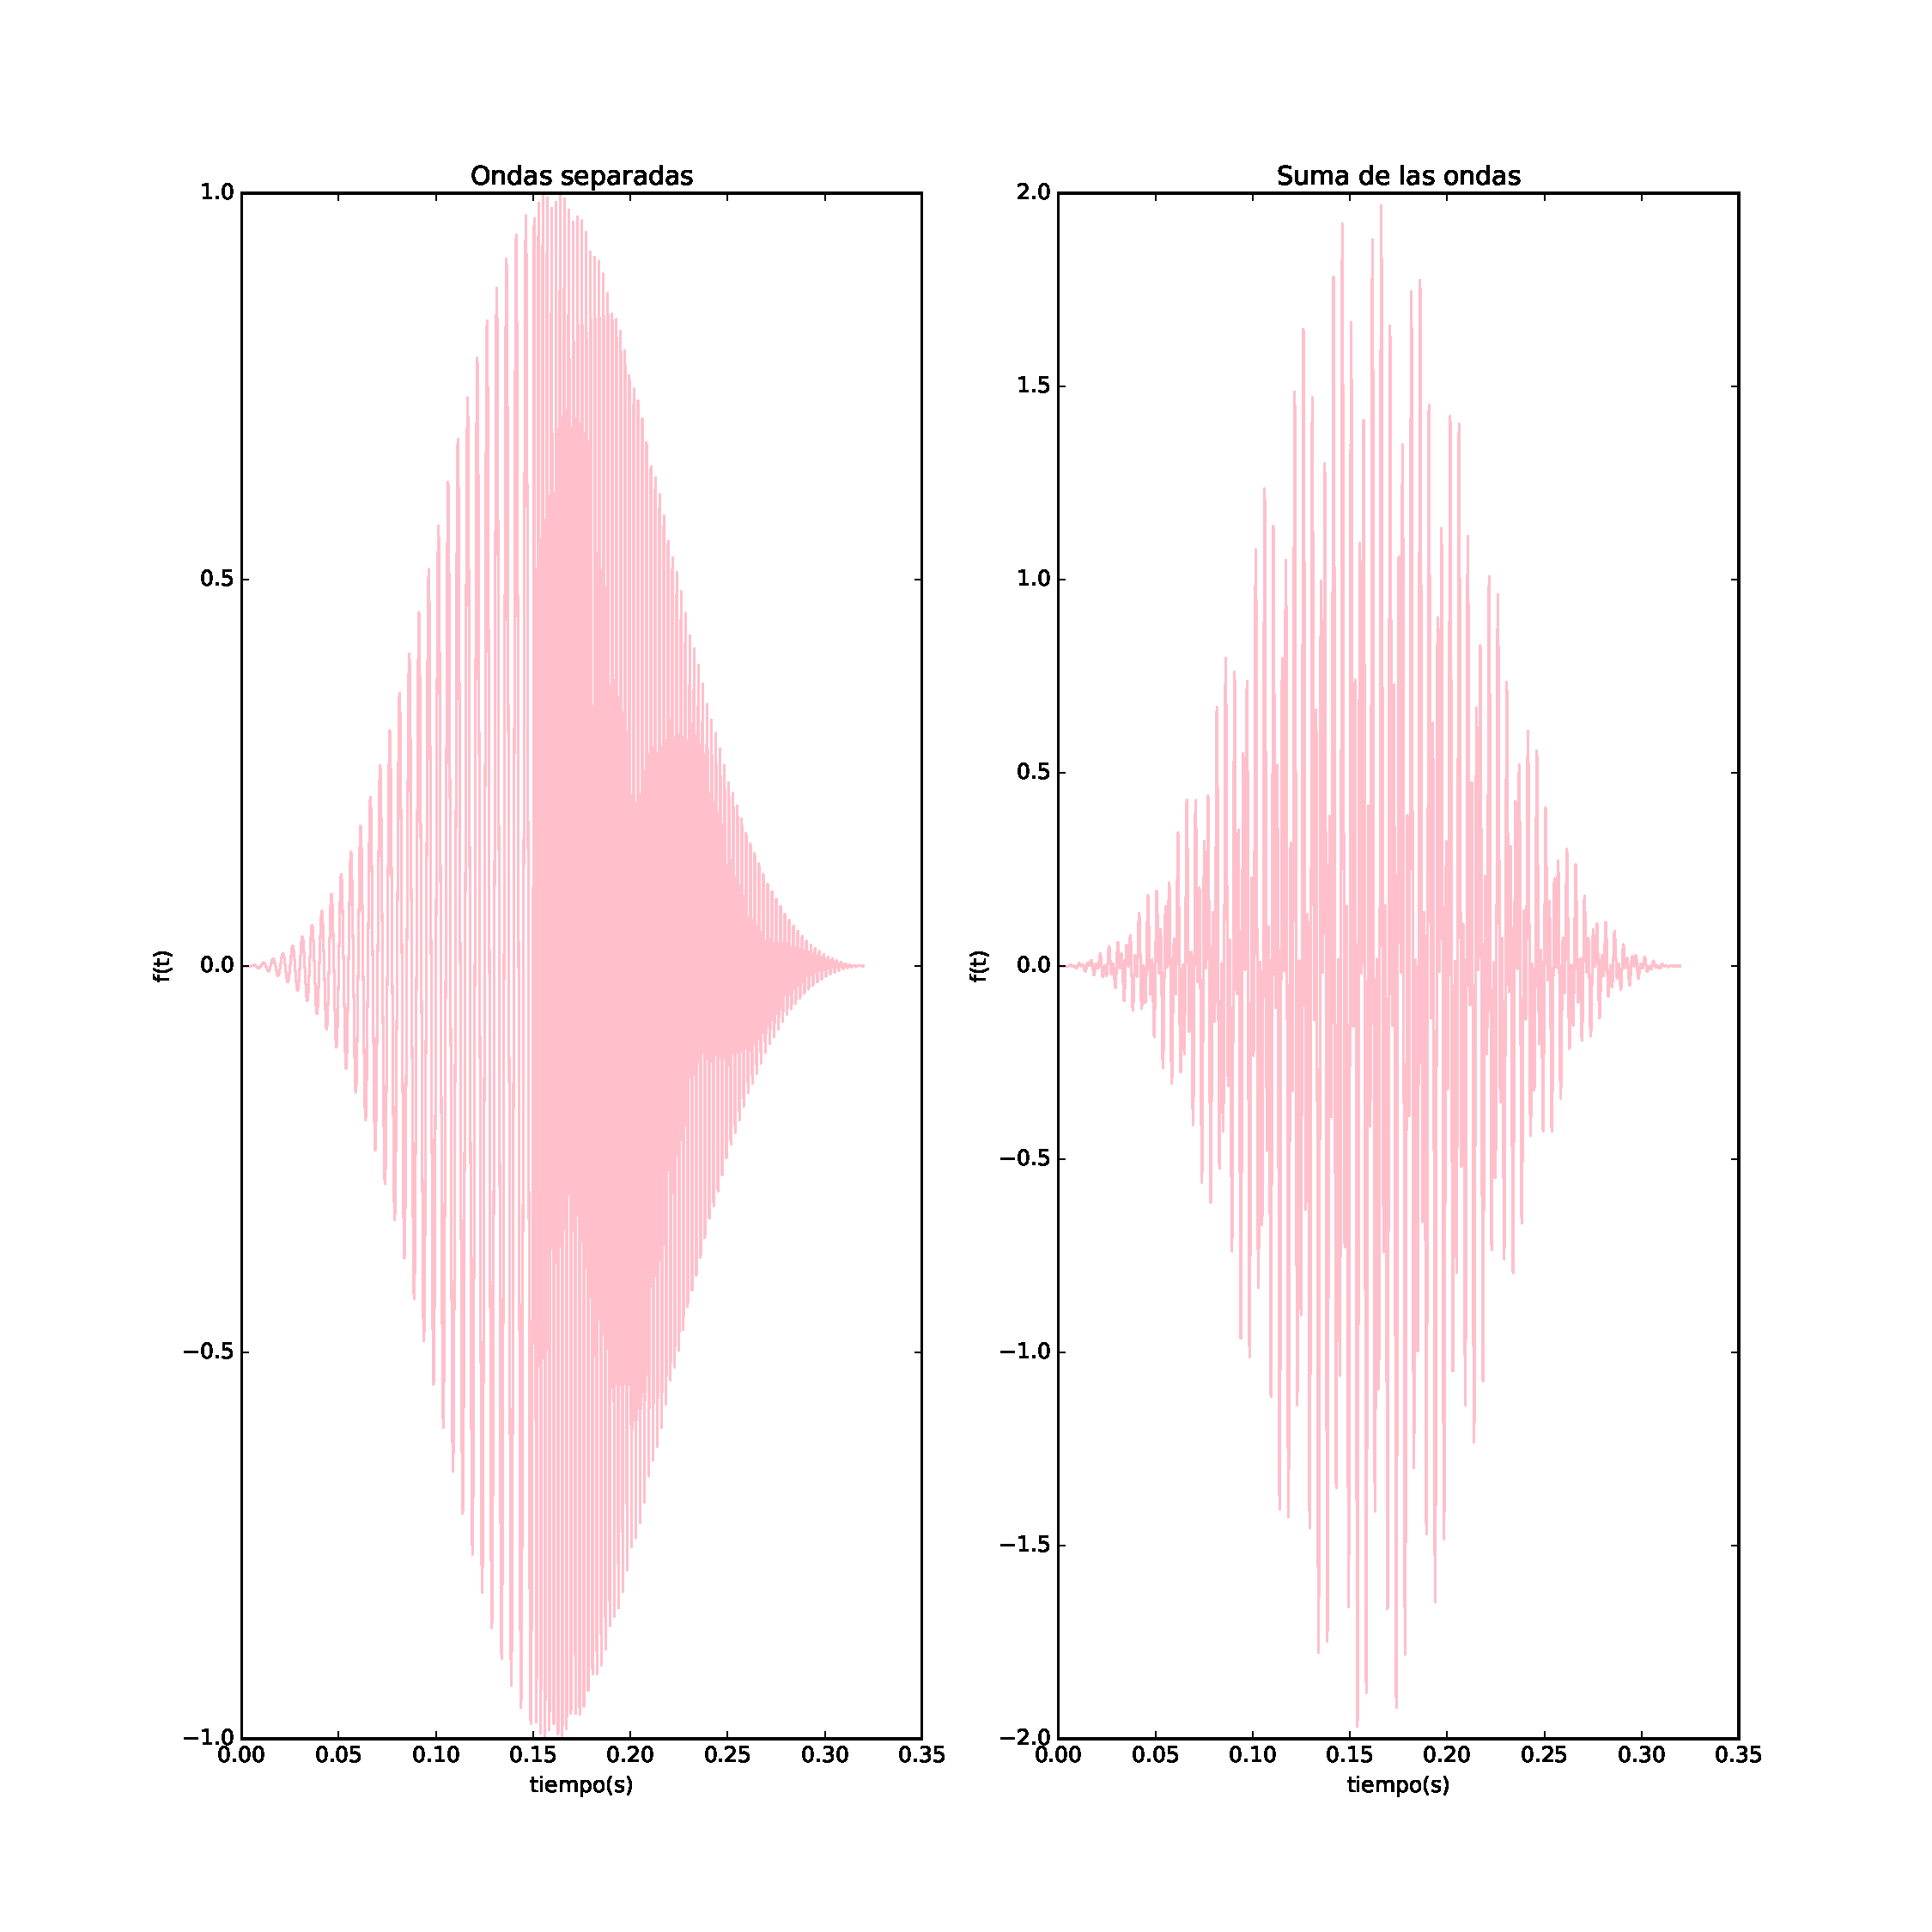
\includegraphics[width=1.1\textwidth]{signals.pdf}
    \caption{Grafica de las seniales.}
    \label{fig:my_label}
\end{figure}
\begin{figure}[H]
    \centering
    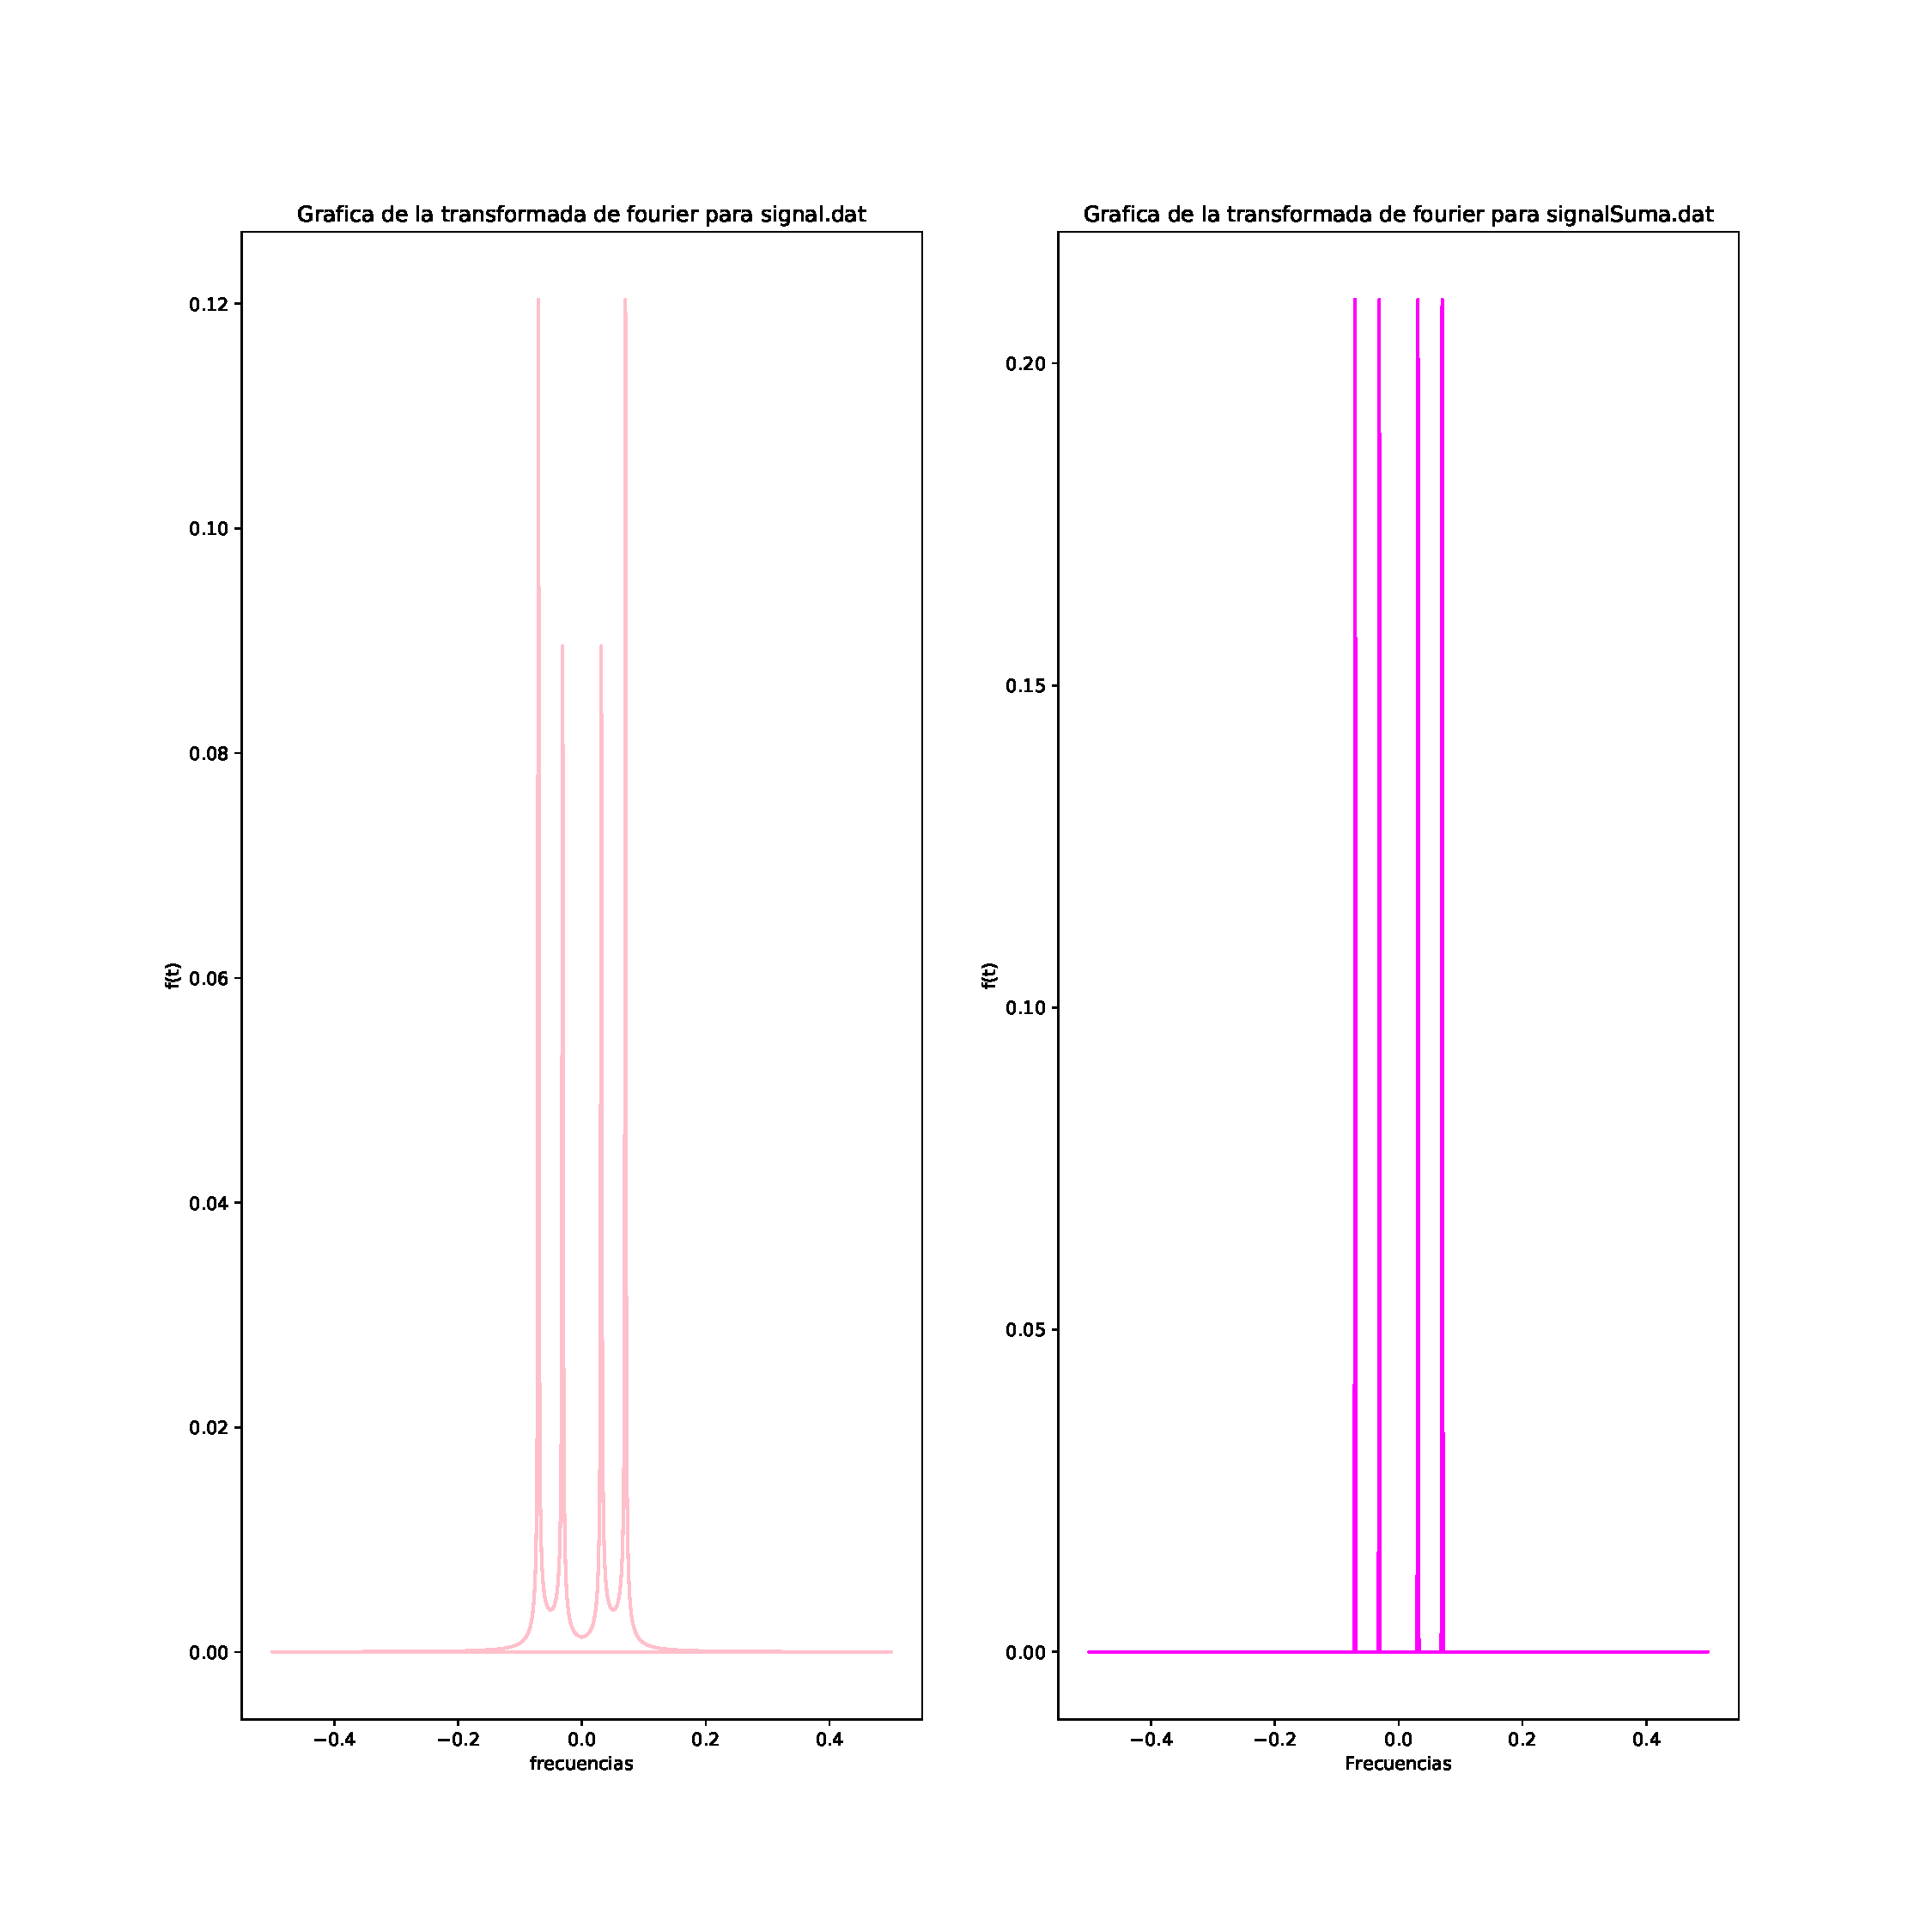
\includegraphics[width=1.1\textwidth]{Fourier_trans.pdf}
    \caption{Grafica de las transformadas de fourier para las dos primeras seniales.}
    \label{fig:my_label}
\end{figure}

\subsubsection{Espectograma}
\subsection{Temblor.txt:}
\begin{figure}[H]
    \centering
    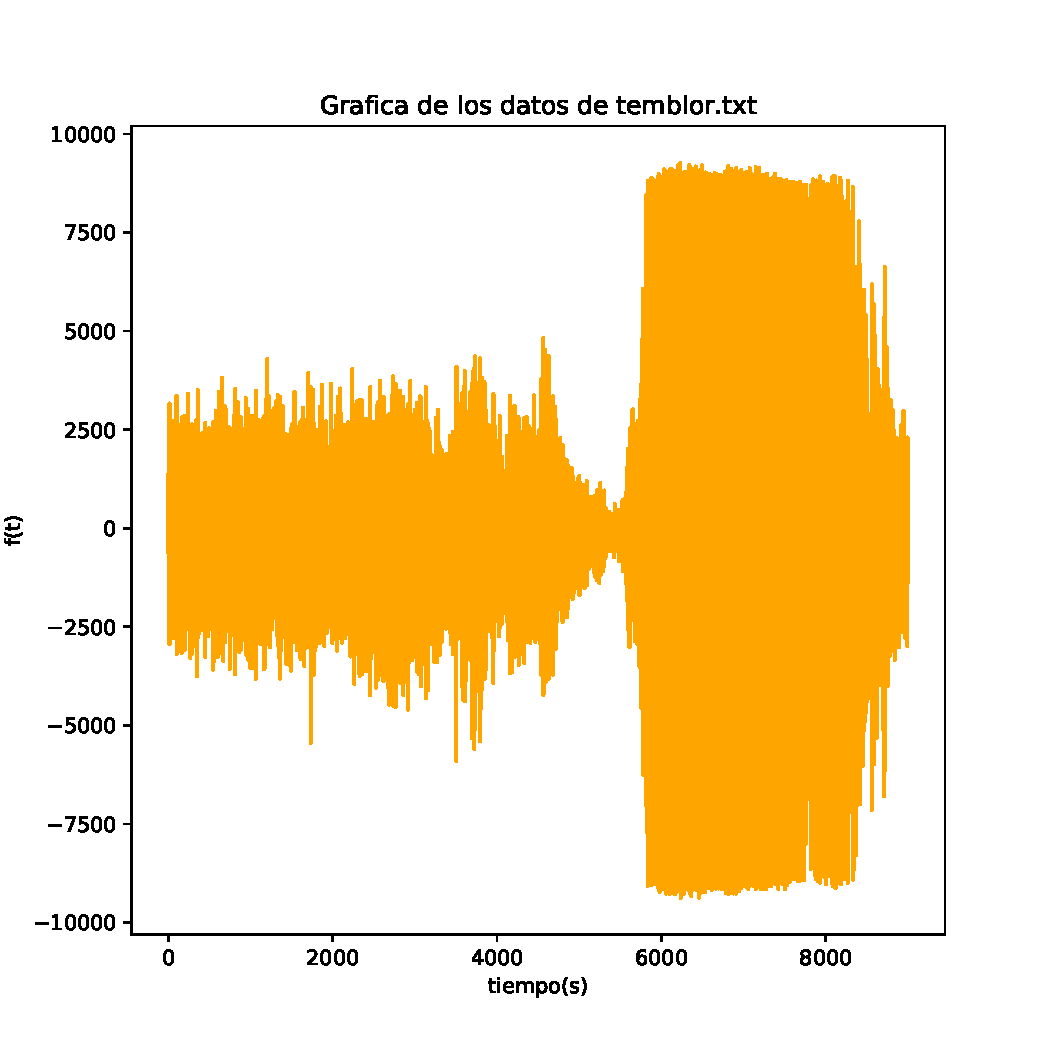
\includegraphics[width=1.1\textwidth]{Temblor.pdf}
    \caption{Grafica de los datos de temblor.txt}
    \label{fig:my_label}
\end{figure}
\begin{figure}[H]
    \centering
    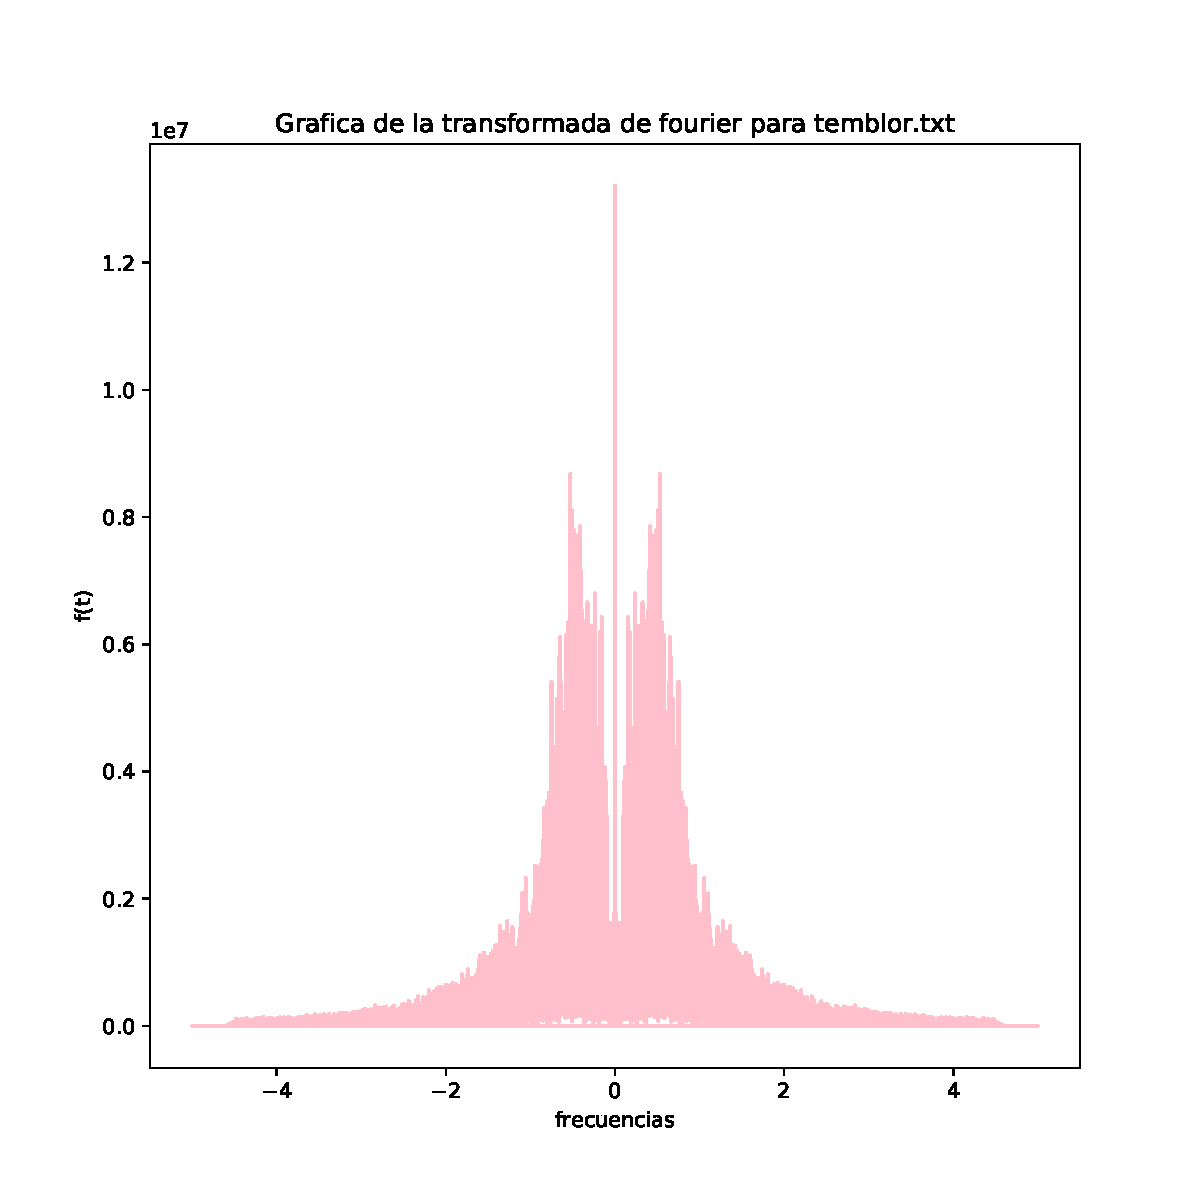
\includegraphics[width=1.1\textwidth]{Fourier_temblor.pdf}
    \caption{Grafica de las transformada de fourier de los datos de temblor.txt}
    \label{fig:my_label}
\end{figure}
\subsubsection{Espectogramas}
\begin{figure}[H]
    \centering
    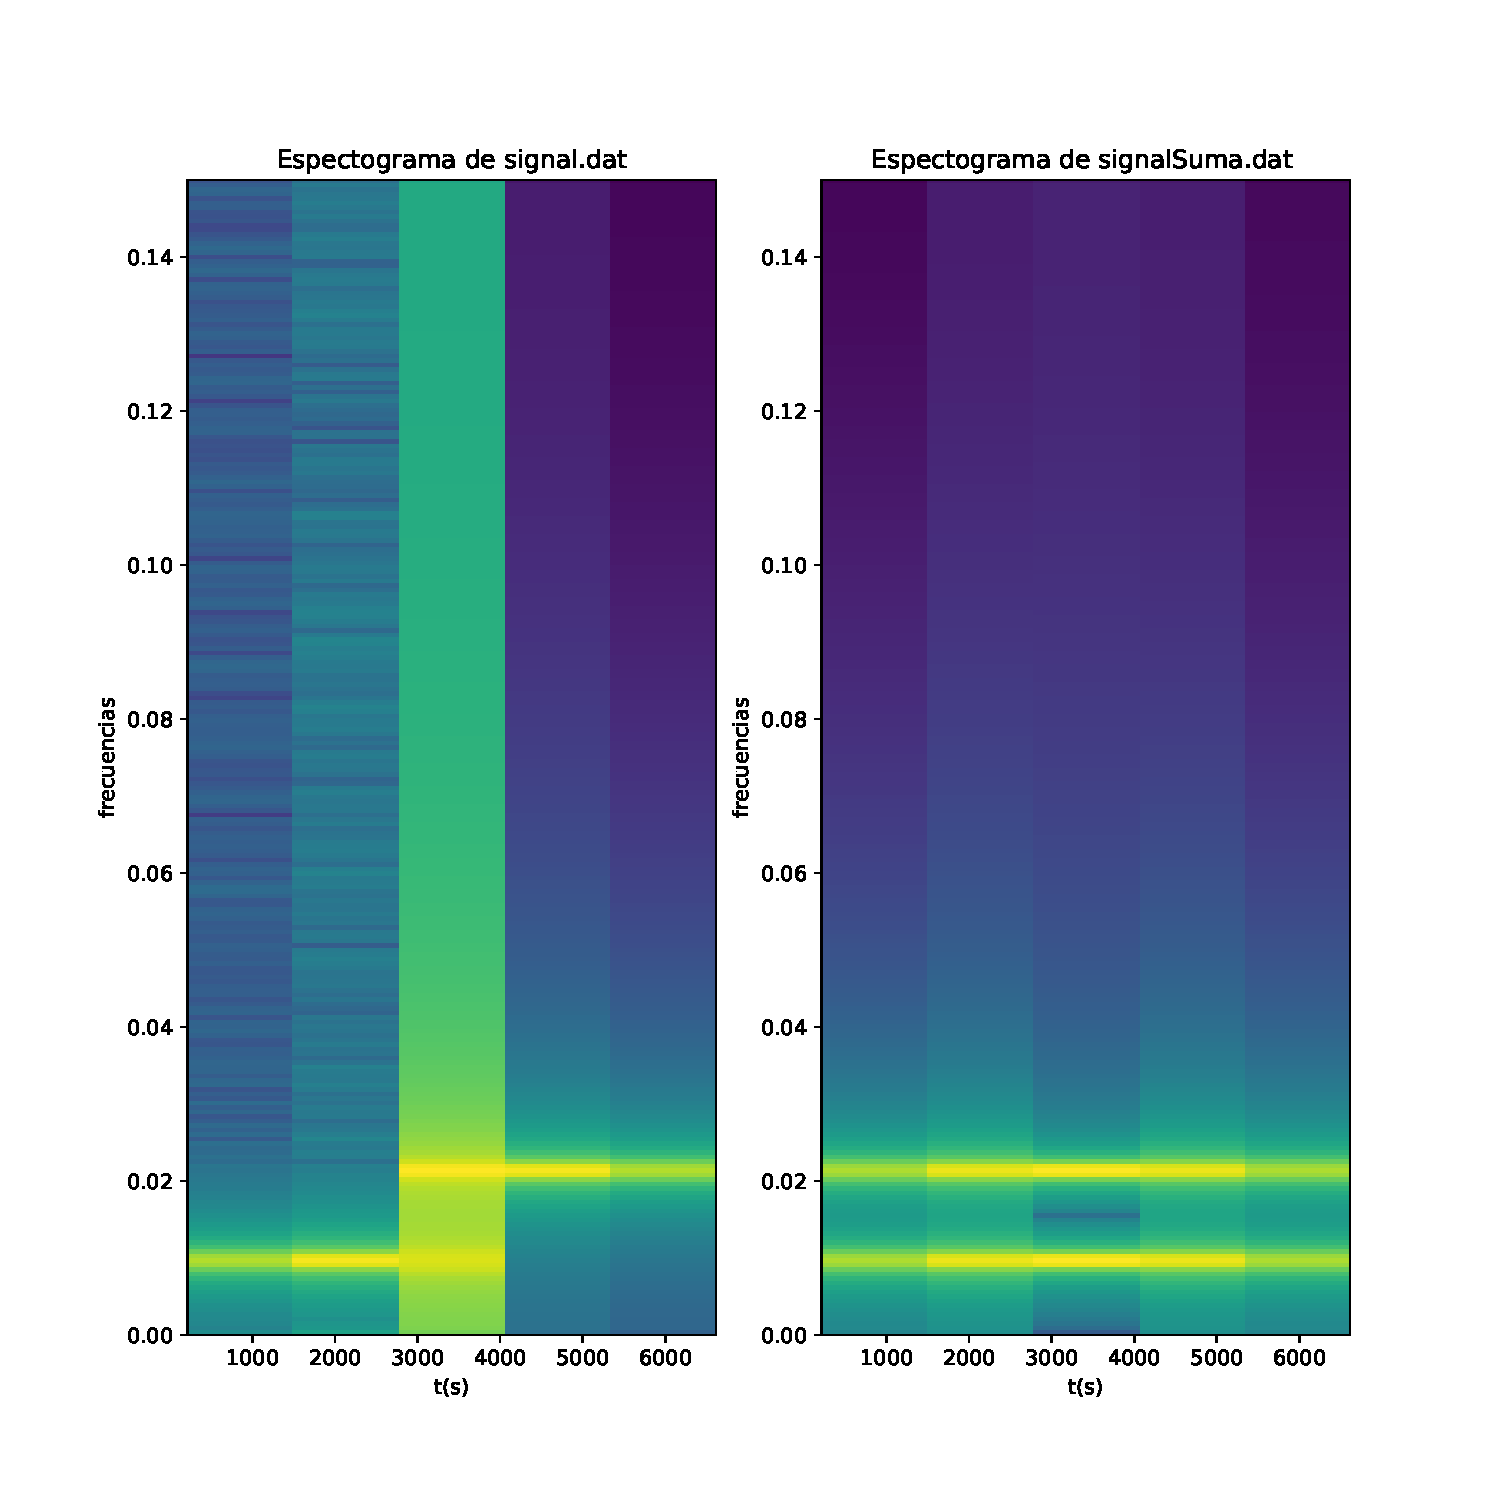
\includegraphics[width=1.1\textwidth]{espectograma.pdf}
    \caption{Espectograma de los datos de las seniales}
    \label{fig:my_label}
\end{figure}
\begin{figure}[H]
    \centering
    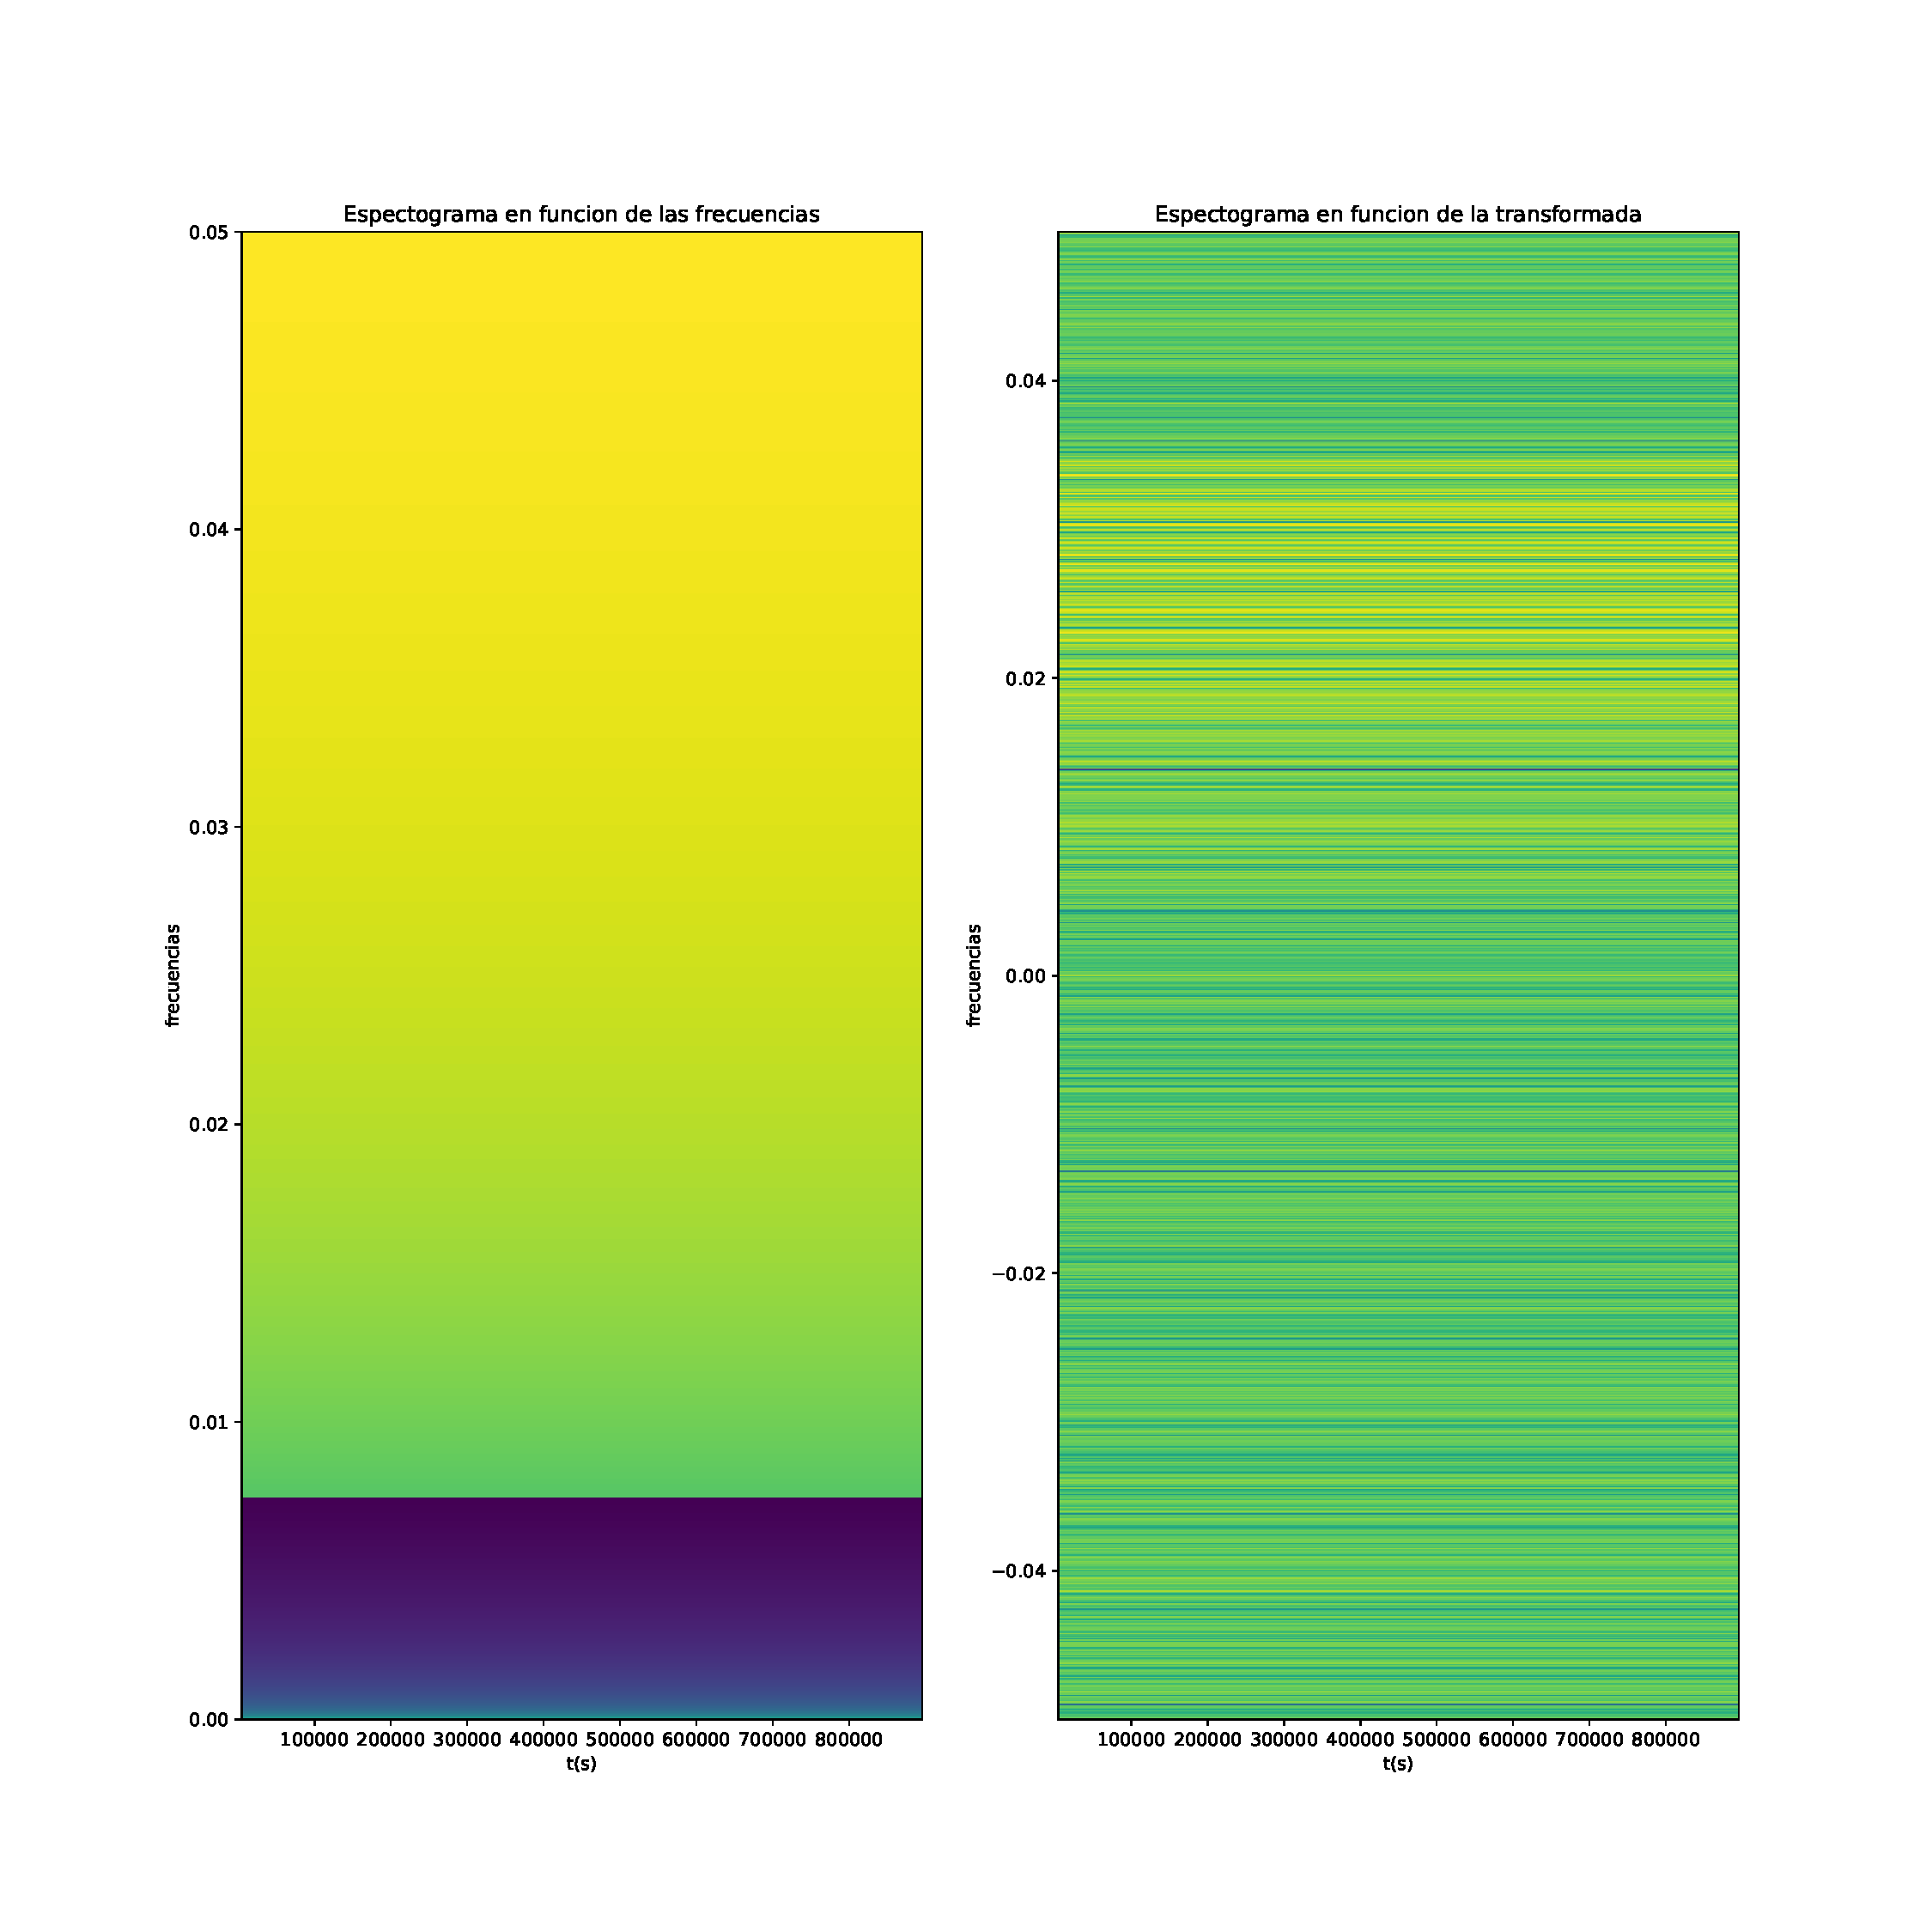
\includegraphics[width=1.1\textwidth]{espectograma_temblor.pdf}
    \caption{Espectograma de los datos de temblor.txt}
    \label{fig:my_label}
\end{figure}
\section{Ejercicio ecuaciones diferenciales}
\begin{figure}[H]
    \centering
    \includegraphics[width=1.1\textwidth]{plot.pdf}
    \caption{primera grafica de ecuaciones diferenciales}
    \label{fig:my_label}
\end{figure}
\end{document}